%!TEX root = main.tex
\section{Data}

The basis of a realistic simulation of global virus outbreak is data on
\begin{itemize}
	\item Geographical population densities
	\item Travel connections (commuting and airports)
\end{itemize}

\subsection{Population}
The population data used in this report comes from NASA \cite{nasa-population}. The data is downloadable in a GeoTIFF file-format which is an image file with population encoded in the pixels.

\begin{figure}[H]
	\centering
	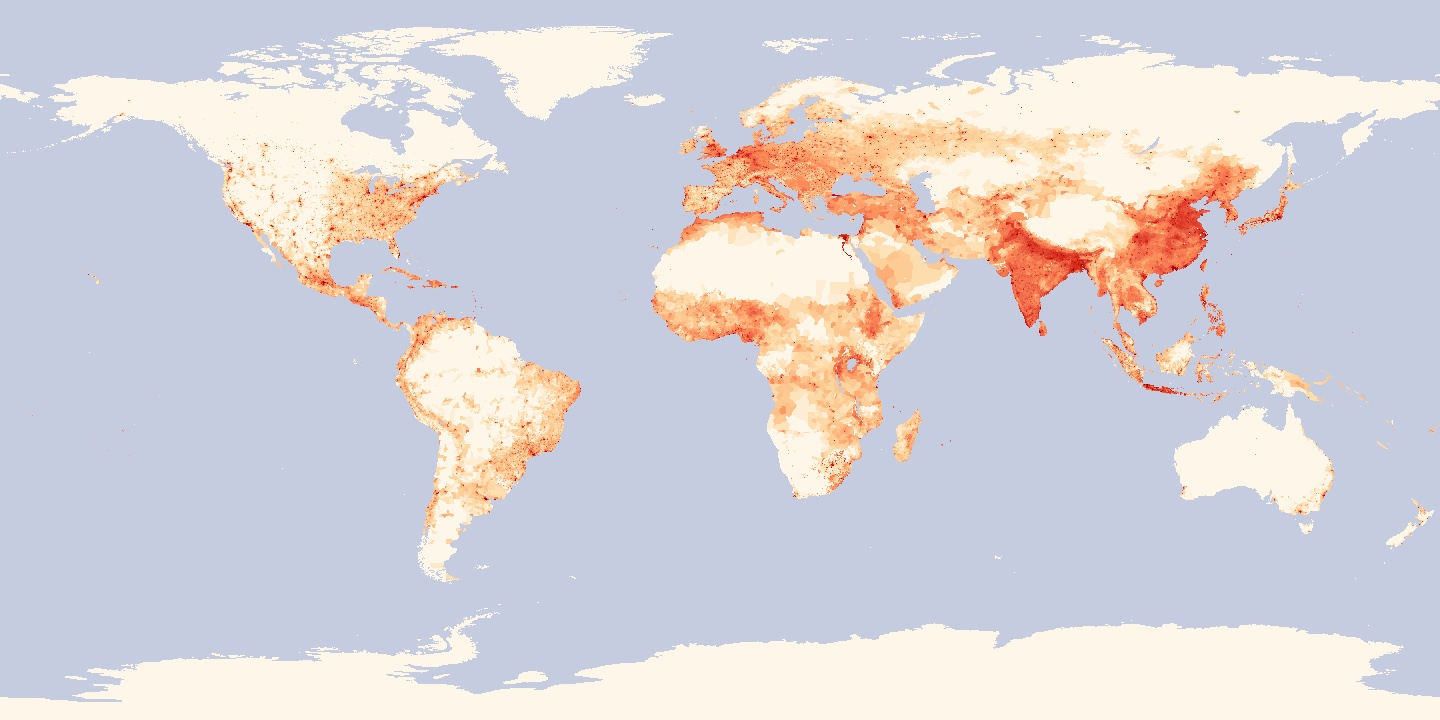
\includegraphics[width=1.0 \textwidth]{plots/nasa_population}
	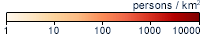
\includegraphics[width=4cm]{plots/nasa_population_colorbar}
	\caption{Plot of population in the world, the used resolution is $0.1 \times 0.1$ degrees per pixel ($3600 \times 1800$).}
\end{figure}

The population dataset encodes $99999.0$ as water and $1.0369266$ as unknown population on land. Thus to get a population map, a raster map of $(x_i < 99999.0 \wedge x_i > 1.0369266) * x_i$ was applied. After this transformation the total world population is just $60,031,128$ (without filtering it is $434,130,384,806$). This is obviously wrong, thus the data is upscaled such the sum is 7.4 billion people.

\subsection{Airport}

The airport connection data was taken from OpenFlights \cite{openflights}. The dataset contains 8021 airports with 37181 airline connections as well as the plane types flying the connection (this could potentially be used for estimating passenger counts). Some the airports did not have any connections and where thus removed.

Plotting the airport connections we see that Europe, East Coast US and East Cost China are the most connected regions. So if a virus spreads takes hold in these areas we would expect it to cause a global outbreak quickly.

\begin{figure}[H]
	\centering
	\includegraphics[width=1.0 \textwidth]{plots/airport_connections.pdf}
	\caption{Plot of all airport connections in the dataset. Because there are so many connections each connection is plotted with a low alpha.}
\end{figure}

\subsection{Aggression}

Based on the location of the airports a Voronoi partition of the of the earths surface is made. From this partitioning one now has geographical regions. The total population of each region can be found by summing over the appropriate pixels in the population dataset. This aggression is the same as done in the GLEaM paper \cite{GLEaM}.

\begin{figure}[H]
	\centering
	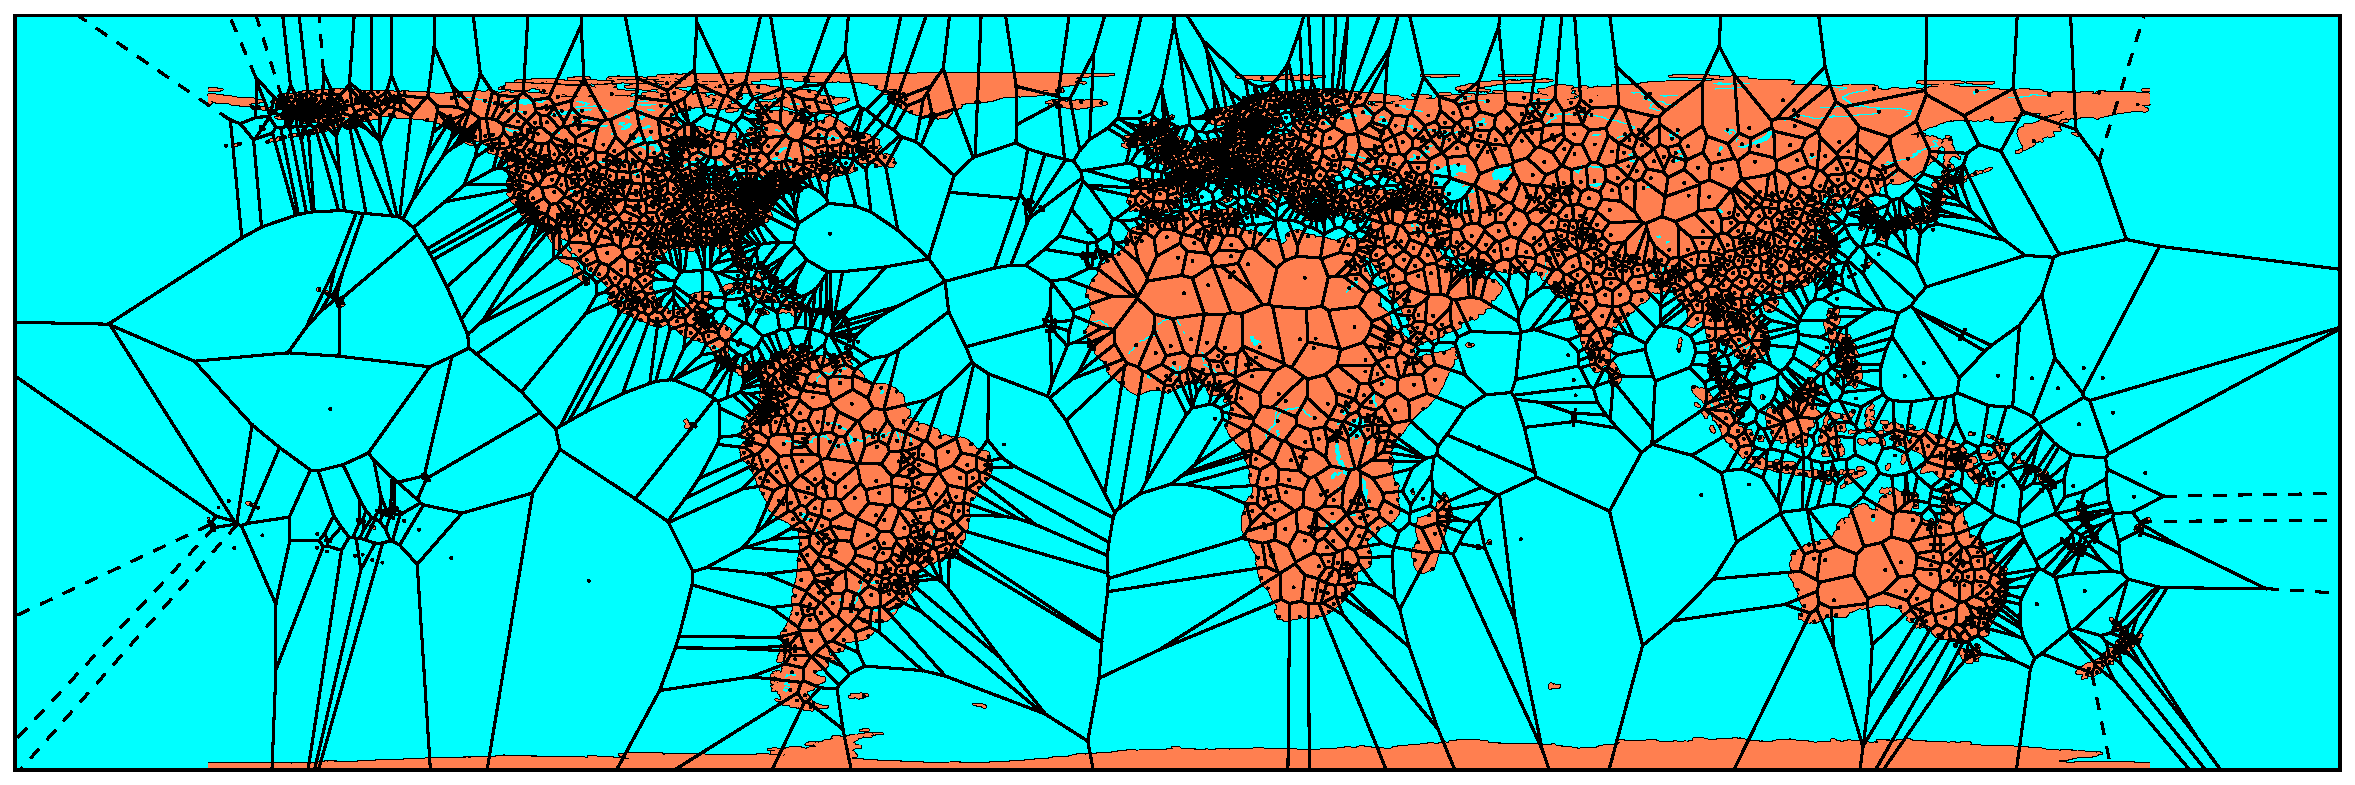
\includegraphics[width=1.0 \textwidth]{plots/voronoi.pdf}
	\caption{Voronoi tessellation based on airport locations. Airports are marked with a dot, region boundaries with lines and dashed lines.}
\end{figure}

